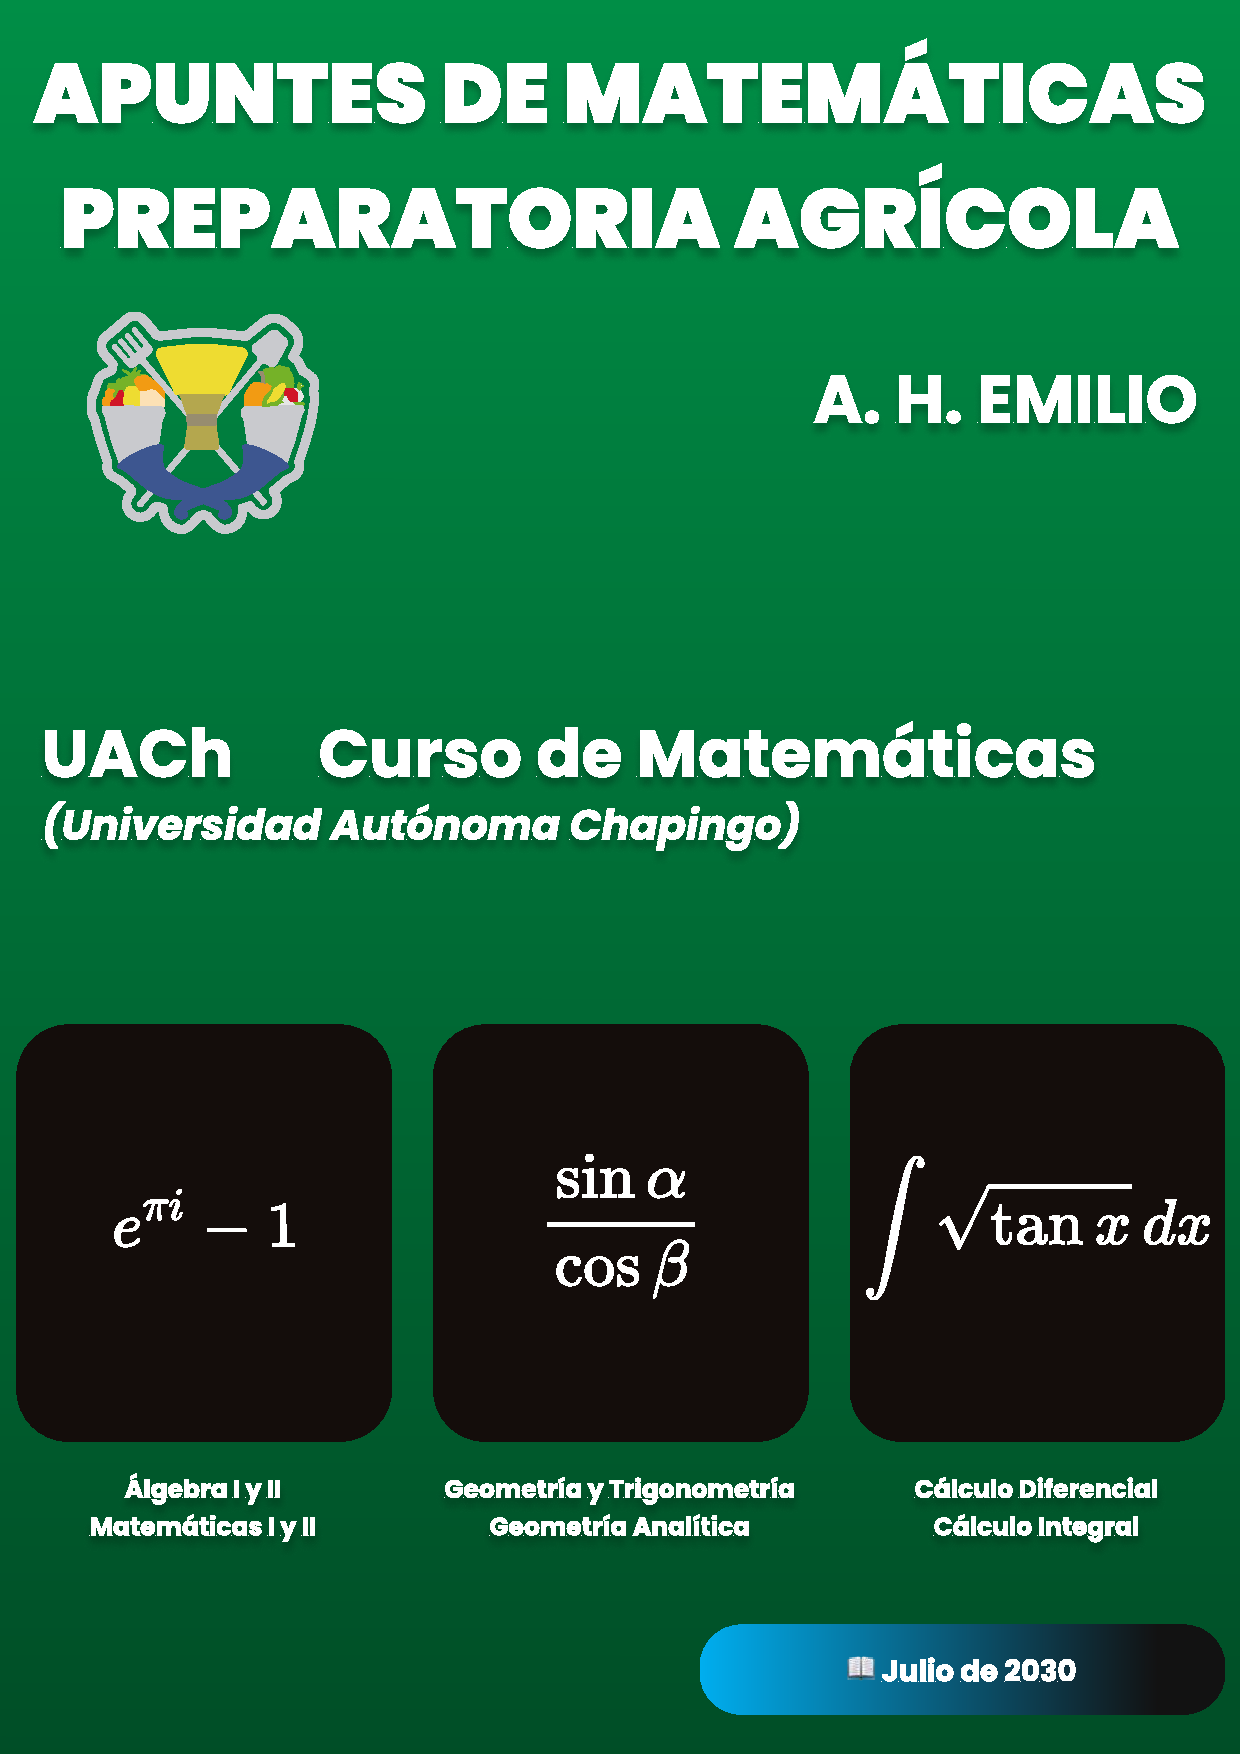
\includepdf[pages=1]{portada.pdf}
%----------------------------------------------------------------------------------------
%	COPYRIGHT PAGE
%----------------------------------------------------------------------------------------
\newpage
~\vfill
\thispagestyle{empty}

\noindent Copyright \copyright\ 2025 Emilio Álvarez Herrera\\ % Copyright notice

\noindent \textsc{Publicado por la Universidad Autónoma Chapingo}\\ % Publisher

\noindent \textsc{Página del autor} \url{https://emilio-ah.web.app}\\ 

\noindent Con licencia de Creative Commons Reconocimiento-No comercial 3.0 Unparted License (la `` Licencia ''). No puede utilizar este archivo excepto de conformidad con la Licencia. Puede obtener una copia de la licencia en \url {http://creativecommons.org/licenses/by-nc/3.0}. A menos que lo exija la ley aplicable o se acuerde por escrito, el software distribuido bajo la Licencia se distribuye en \textsc{`` tal cual '', sin garantías ni condiciones de ningún tipo}, ya sea expresa o implícita. Consulte la Licencia para conocer el idioma específico que rige los permisos y las limitaciones de la Licencia.\\ % License information

\noindent \textit{Primera edición, \today} % Printing/edition date (Noviembre del 2020)

%----------------------------------------------------------------------------------------
%	TABLE OF CONTENTS
%----------------------------------------------------------------------------------------

%\usechapterimagefalse % If you don't want to include a chapter image, use this to toggle images off - it can be enabled later with \usechapterimagetrue

%%%%%%%%%%%%%%%%%%%%%%%%%%%%%%%%%%%%%%%%%%%%%%%%%%%%%%%%%%%%%%%%%%%%%%%%%%%%%%%%%%%%%%%%%%%%%%%%%%%%%%%%%%%%%%%%%%%%%%%%%%%%%

\chapterimage{2.pdf} % Table of contents heading image

\pagestyle{empty} % No headers

\tableofcontents % Print the table of contents itself

\cleardoublepage % Forces the first chapter to start on an odd page so it's on the right

\pagestyle{fancy} % Print headers again